\documentclass[12pt]{article}

%-------Packages---------
\usepackage{enumerate}
\usepackage[margin=0.75in]{geometry}
\usepackage{rotating}
\usepackage{hyperref}
\usepackage{verbatim}
\usepackage{amsthm}

\bibliographystyle{plain}

\newtheorem{lemma}{Lemma}


%--------Meta Data: Fill in your info------
\title{Max Flow in a Directed Planar Graph}
\date{\today}
\author{Jason Hoch and John Wang \\
6.854 Final Paper}


\begin{document}

\maketitle

\abstract{Maximum flow is a classical problem in computer science and many incremental improvements have been made in the last decade. However, few authors have attempted to examine the practical results of many of these algorithms. We provide insight into max-flow implementations in industry. In particular, we examine the maximum flow problem on directed planar graphs, since they seem to have the most practical application. We implement an $O(n \log n)$ algorithm presented by Erickson 2010 \cite{erickson2010} and examine its runtime in comparison with standard max-flow algorithms. We also examine the theoretical and practical implications of using a naive spanning tree data structure, instead of the top-tree data structure suggested in \cite{erickson2010}, as a subprocedure in the algorithm. We find that the naive implementation outperforms the more complicated top tree structure in small to medium sized graphs.}

\tableofcontents

\newpage

\section{Introduction}

The general maximum flow problem has many applications in operations research and supply chain management. The classic algorithms used to solve the problem are polynomial, but relatively slow. The Edmonds-Karp algorithm requires $O(n m^2)$ time, while Ford Fulkerson requires $O(m \max |f|)$. Improvements made throughout the last few decades have decreased these runtimes by using concepts from blocking-flow and push-relabel algorithms. Dinitz's blocking flow algorithm improved the runtime to $O(n^2 m)$ by using a breadth-first-search in the residual graph to build a layered graph \cite{dinitz1970}. Goldberg and Tarjan \cite{goldbergtarjan1986} introduced a general framework for solving max-flow problems by using the idea of push relabel. Many of the fastest algorithms for maximum flow are variants of this general framework. Recently, Orlin presented an algorithm which runs in $O(nm)$ time. 

A practical application of a maximum flow algorithm, however, would find many of these algorithms prohibitively slow. Even the best known algorithm of Orlin for general graphs is $o(n^2)$ for reasonably connected graphs. However, these algorithms perform poorly due to their generality. In practice, only a certain subset of graphs are likely to arise. For instance, in many applications of maximum flow, it is reasonable to assume that the graphs will be planar. 

This is the case for most maximum flow networks on a two dimensional map. In these cases, solving the problem in its full generality does too much work, and enforcing constraints on the assumptions of the graph can improve runtime. This paper focuses on the algorithm proposed by Erickson 2010 \cite{erickson2010}, which exploits planarity to achieve $O(n \log n)$ runtime. This significantly reduces the execution time of the algorithm, at least theoretically.

This paper implements the Erickson algorithm and presents the observed runtime on a set of planar graphs. The set of planar graphs generated contains graphs of varying sizes. Our implementation of the Erickson algorithm is tested for how it scales with $n$, the number of vertices in a graph. We attempt to determine an empirical function for how the observed runtime scales with $n$, and compare it with an asymptotically weaker implementation of max-flow, namely Edmonds-Karp.

The rest of the paper presents a brief overview of the Erickson algorithm, the unique features in our implementation, and the object oriented infrastructure we created. We present the results from our implementation on a set of planar graphs and compare it with standard maximum flow algorithms.

\section{Motivation}

In this section, we provide motivation for our implementation. In particular, we motivate the use of an algorithm specific to planar graphs. We argue that most applications of maximum flow are constrained to planar graphs, and hence, that the Erickson algorithm provides a non-trivial improvement upon past algorithms. 

\subsection{Supply Chain Example}

First, suppose a chain of department stores has a supply chain and is attempting to find the best way to move goods from its production facilities to its stores. One subproblem of this is that the store must transport goods across the network from a particular production facility to a particular store. There are a discrete number of warehouses that its trucks can stop at and a discrete number of trucks that it sends over any route. Since this production facility and store pair is not isolated in its global network, the chain cannot add or remove any trucks or change any routes. The goal is to achieve the highest throughput of goods possible from the production facility to the store.

This problem can be reduced to a single source, single sink maximum flow problem in planar graph. If trucks are allowed to stop and readjust their loads at intersections of large highway networks, then there exists a planar embedding of this problem onto a two-dimensional graph. Placing a warehouse at intersections of large highways is also not very restrictive, since most retail chains rent out retail space from a large supplier. In other transportation problems, these can be thought of as large distribution centers such as ports or airports from which the company can rent out space for a low fixed cost. 

Notice that this type of transportation problem occurs with incredible frequency. Every large chain of stores with a need to move goods across land has a similar problem. Retailers such as Amazon, Walmart, and Target have a large incentive to optimize their transportation networks, as do large shipping companies such as FedEx and UPS. 

\subsection{Computer Vision Example}

There are also many examples of planar max-flow networks which are relevant in computer vision. In particular, finding graph cuts in an image is a widely used industrial application of max-flow. Greig, Porteous, and Seheult \cite{greigporteousseheult1989} provide an example of using max-flow for smoothing noisy images. They show that the maximum a posteriori estimate of a noisy image is given exactly by finding a max-flow in a specifically defined image network. 

The authors in \cite{greigporteousseheult1989} create a network of pixels $i$, each with value $x_i \in \{0,1\}$ corresponding to white and black. Each pixel $i$ in the flow network has neighbors which are the pixels touching it in the actual image. The capacity of the edge between pixels $i$ and $j$ is defined as a log-likelihood ratio corresponding to the probabilitiy that the values of pixels $i$ and $j$ are correct. The paper shows that finding a maximum flow through the network results in a maximum a posteriori estimate of the image. 

The network is clearly planar because the graph can be embedded onto a two dimensional plane (the image). Moreover, \cite{greigporteousseheult1989} spawned a large literature in the computer vision field using max-flows as a means to separate out nosie from images. Other max-flow algorithms in the computer vision field follow in a similar vein to \cite{greigporteousseheult1989}. 

\section{Overview of Erickson's Algorithm}

This section provides an overview of the Erickson algorithm. We summarize the main results from the paper in \cite{erickson2010} and sketch the proofs of the main theorems. The Erickson algorithm relies on the observation that max-flow in directed planar graphs can be reformulated as a parametric shortest paths problem. The algorithm finds a parametric shortest paths spanning tree whose parameter is perturbed in multiple iterations of the algorithm. Eventually, the resulting tree will arrive at a state where the max-flow can be computed with simple arithmetic. 

\subsection{Definitions}

First, we shall present the fundamental definitions and terminology used throughout the this paper and the Erickson \cite{erickson2010} paper. Note that the notation is the same as in \cite{erickson2010} to reduce confusion. A graph $G = (V,E)$ will be a directed planar graph where each edge $e$ denoted as $u \to v$ contains a head and tail defined as $head(e) = v$ and $tail(e) = u$ respectively. The reversal of the graph is defined as $rev(e) = head(e) \to tail(e)$. 

Each primal graph $G$ has a corresponding dual $G^*$ where each primal face is converted into a dual vertex. Two dual vertices are connected by a dual edge if and only if there is a corresponding primal edge connecting the two faces represented by the two dual vertices. In particular, consider faces $a$ and $b$ in the primal graph, and consider some edge $e$ which separates these two faces. Then the dual graph will contain an edge $e^*$ (the dual of the edge $e$) which is oriented $90^\circ$ counterclockwise to $e$ and connects $a^*$ and $b^*$ in the dual. 

A flow between source $s$ and sink $t$ is defined as a function $\phi : E \to \mathrm{R}$. The flow satisfies antisymmetry and conservation. In particular, the antisymmetric constraint specifies that $\phi(e) = -rev(\phi(e))$ while the conservation constraint specifies that $\sum_{e_w} \phi(e) = 0$ for all edges $e$ such that $w = head(e)$. We define a feasible flow by defining a non-negative capacity function $c : E \to \mathrm{R}$ on each edge $e$. For a flow to be feasible on a graph, we must have $\phi(e) \leq c(e)$ for all edges $e$ in the graph. 

\subsection{Parametric Shortest Paths}

Before moving on to Erickson's algorithm, it is instructive to examine the parametric shortest paths problem, since Erickson's algorithm is fundamentally based on the idea of using parametric shortest paths to compute the max-flow. For this problem, consider a graph $G = (V,E)$ and an additional parameter $\lambda$. We define a new cost function $c : E \to \mathrm{R}$ and obtain a subset $E' \subset E$ of the edges of the graph. The cost function will be set to $c(\lambda, e) = c(e) - \lambda$ for all edges $e \in E'$ and $c(\lambda, e) = c(e)$ for all edges $e \notin E'$. The parametric shortest paths problem asks to compute the largest value of $\lambda$ for which the resulting graph with weights $c(\lambda, e)$ has no negative-weight cycles. 

A number of algorithms that solve this problem use the concept of a pivot tree. Young, Tarjan, and Orlin \cite{youngtarjanorlin1991} solve the problem in $O(nm + n^2 \log n)$ by constructing a single-source shortest paths tree. The distance used in the shortest paths tree is equal to the cost $c(\lambda, e)$ for each edge $e$, given a parameter $\lambda$. The Young, Tarjan, and Orlin algorithm starts increasing $\lambda$ from $-\infty$. At some point, $d(\lambda, v) = d(\lambda, u) + c(\lambda, v)$ for some edge $u \to v$ which is not in the shortest paths tree. When this occcurs, the shortest paths tree incorporates the $u \to v$ edge and removes an appropriate edge $e$ where $head(e) = v$ so that the tree remains a valid shortest paths tree. The algorithm continues until a cycle appears in the tree. Notice that at this point, increasing $\lambda$ by any amount will cause a negative-weight cycle in the original graph because the cycle must be of weight 0. 

This algorithm therefore computes the maximum $\lambda$ for which the graph $G$ has no negative-weight cycles. Erickson's algorithm will use the same concept and apply it to max-flow. In particular, Erickson uses the parameter $\lambda$ to pivot edges in a shortest paths tree. Using a well defined set of weights, one can show that the resulting algorithm solves the max-flow problem.

We also define the dual residual network $G^*_\lambda$ of some graph $G$ for some parameter $\lambda$. It is defined on the dual graph $G^*$ and has a cost function $c : \mathrm{R} \times E^* \to \mathrm{R}$ where $c(\lambda, e^*) = c(\lambda, e)$. Note that the edge $e$ is well defined since each edge $e$ has a corresponding dual edge $e^*$ which is $90^\circ$ counterclockwise from $e$ and connects the faces which $e$ separates. Notice that each edge $e^*$ corresponds to exactly one edge, so taking the cost on the primal edge $c(\lambda, e)$ is well defined for each dual edge $e^*$. 

\subsection{Erickson's Algorithm}

The algorithm that Erickson provides in \cite{erickson2010} first creates a shortest-paths tree, then runs a parameterized shortest-paths algorithm. It uses a dynamic tree data structure to find pivots and remove them from the tree. To explain this algorithm, we start by examining co-cycles. Let $P$ be a path from $s$ to $t$ in the primal graph, and set $\pi : E \to \mathrm{R}$ be a unit flow function. We set $\pi(e) = 1$ for $ e \in P$, $\pi(e) = -1$ for $rev(e) \in P$, and $\pi(e) = 0$ otherwise. Now define a co-cycle as some subgraph $C \subset G$ for which its dual $C^*$ is a simple directed cycle in $G^*$. Let $\pi(C) = \sum_{e \in C} \pi(e)$ be called the crossing number. Erickson shows that the crossing number is confined to the values $\{-1,0,1\}$ for any co-cycle $C$. 

First, if $n_{plr}$ is the number of times that $P$ crosses $C^*$ from left to right and $n_{prl}$ for the opposite direction, Erickson shows that $\pi(C) = n_{plr} - n_{prl}$. This means that one can break down the calculation of $\pi(C)$ into cases. Erickson invokes the Jordan Curve Theorem and asserts that any co-cycle's dual $C^*$ must partition the dual into two halves. If $s$ and $t$ lie in the same half, then the number of times that $P$ crosses $C^*$ from left to right is equal to the number of times it crosses from right to left since it must eventually reach $t$ again. Therefore, $\pi(C) = 0$ in this case. In the second and third cases, $s$ and $t$ lie on different halves, so either $n_{plr} = n_{prl} + 1$ or $n_{plr} + 1 = n_{prl}$, depending on the orientation of $s$ and $t$ in the halves. This means that $\pi(C) = \pm 1$ in these two cases. This shows that $\pi(C) \in \{-1,0,1\}$.

Moreover, Erickson shows that every $(s,t)$ cut has $\pi(C) = 1$, since $P$ contains one extra edge in $C$ than in $rev(C)$ (by the fact that $n_{prl} = n_{plr} + 1$). Now if $C$ were not an $(s,t)$ cut, then there would be some path from $s$ to $t$ which did not go through $C$. Since the original $P$ has one extra edge in $C$ than in $rev(C)$, this cannot be the case, so $C$ must be an $(s,t)$ cut.

Now, if one thinks about the residual network $G^*_\lambda$, one can see that $\lambda$ serves as something akin to a parameter in linear programming, in the sense that its feasibility in the dual immediately corresponds to the feasibility of a flow in the primal with value $\lambda$. By feasibility in the dual, we mean to say that the shortest paths distances induced by the costs $c(\lambda, e^*) = c(e) - \lambda \pi(e^*)$ have no negative weight cycles. Erickson formalizes this with lemma \ref{lem:resid-network}.

\begin{lemma}
There exists a feasible $s-t$ flow in $G$ with value $\lambda$ if and only if the dual residual network $G^*_\lambda$ does not contain a negative cycle. 
\label{lem:resid-network}
\end{lemma}

Lemma \ref{lem:resid-network} follows because of our insight that $\lambda \in \{-1,0,1\}$. Suppose $G^*_\lambda$ contains a negative-weight cycle. Then one can decompose the cycle into its constituent edges. This implies that for a negative weight cycle $C^*$, one must have $\sum_{e \in C^*} c(e) - \lambda \pi(C) < 0$ by the definition of the costs. This means that $\pi(C) > 0$ since $c(e) \geq 0 \forall e$ and $\lambda \geq 0$. However, from our previous result, we know that $\pi(C) > 0$ implies that $\pi(C) = 1$, which occurs exactly when $C$ is an $(s,t)$ cut. This cut $C$, with capacity less than $\lambda$, does not allow for a feasible flow of value $\lambda$, since there is no possible way of getting from $s$ to $t$ without going over the cut (which does not have enough capacity). 

Now, we see that the maximum flow in the graph will be given by the maximum feasible $\lambda$, called $\lambda_{max}$. This is because there always exists a flow of value $\lambda$ in the primal graph when $G^*_\lambda$ does not have a negative cycle. Therefore, the largest possible flow occurs for $G^*_{\lambda_{max}}$, or the crtical value of $\lambda$ which introduces a negative weight cycle into $G^*$. To show this, suppose there existed some flow of value $f > \lambda_{max}$. Then, it must be feasible so that by lemma \ref{lem:resid-network}, $G^*_f$ does not contain a negative cycle. However, this implies that $f > \lambda_{max}$ is a value of $\lambda$ for which $G^*_\lambda$ has no negative weight cycles, which is a contradiction.

The Erickson algorithm computes $T_\lambda$, which is the shortest paths tree with parameter $\lambda$, computed on $G^*_\lambda$. For clarification, the shortest paths tree uses the cost $c(\lambda, e)$ as a measure of distance. Lemma \ref{lem:directed-cycle} shows how everything connects together to create an algorithm.  

\begin{lemma}
$\lambda_{max}$ is the first critical value of $\lambda$ whose pivot introduces a directed cycle into $T_{\lambda}$. 
\label{lem:directed-cycle}
\end{lemma}

The Erickson algorithm computes an intial spanning tree $T_0$, and begins to increase the value of $\lambda$. At some point, a directed cycle will be created inside of $T_\lambda$ due to lemma \ref{lem:directed-cycle} (we won't give a proof, but it can be found in \cite{erickson2010}). However, we know that by lemma \ref{lem:resid-network}, the $\lambda_{max}$ value at which a directed cycle in $T_{\lambda_{max}}$ occurs is exactly the value of the maximum flow in the primal.

A surprising feature of Erickson's algorithm is that it does not deal at all with flows in the primal graph. Instead, it does all its work in the primal, and particularly in the shortest-paths spanning tree $T_{\lambda}$. The complexity of the algorithm comes from building and maintaining the spanning tree $T_{\lambda}$ while inserting and removing edges (pivots). Moreover, notice that in each iteration, one needs to be able to increase $\lambda$ and build a new shortest paths spanning tree. 

In essence, Erickson's algorithm provides an efficient way for recomputing the spanning tree at each iteration. Erickson uses the fact that the spanning tree changes only minimally when a single edge is pivoted. Below we present the pseudocode and refer the reader to Erickson \cite{erickson2010} for details and motivation for how each step of the algorithm fits into the picture we have described above.

\subsection{Formalized Algorithm}

To make the above overview more formal, the pseudocode for Erickson's algorithm is provided below. First, however, we define the distance $dist(\lambda, p)$ for a vertex $p$ in the dual with parameter $\lambda$ as the shortest path distance from some arbitrary starting node $o$ to $p$. Note that the shortest path distance is computed over the cost function $c(\lambda, e^*) = c(\lambda, e)$ as defined earlier in the paper (each dual edge retains the cost function of its primal). We define slackness on an edge $e^* = u \to v$ in the dual with parameter $\lambda$ as $slack(\lambda, e^*) = dist(\lambda, u) + c(\lambda, e^*) - dist(\lambda, v)$. 

The slackness of an edge in the dual provides a basis for how pivots in the shortest paths tree are introduced. In particular, Erickson notes that the algorithm has an invariant which keeps $slack(\lambda, e^*) = 0$ exactly when $e^* \in T_{\lambda}$ or when $\lambda$ is a critical value corresponding to a new pivot. 

We are now ready to present Erickson's algorithm in pseudocode (taken from Erickson \cite{erickson2010}):
\begin{quote}
\begin{verbatim}
PlanarMaxFlow(G, c, s, t):
    Initialize spanning tree L
    While s and t are in the same component of L:
        LP = path in L from s to t
        min_edge = edge in LP* with minimum slack
        d = slack(min_edge)
        forall edges e in LP:
            slack(e*) = slack(e*) - d
            slack(rev(e*)) = slack(rev(e*)) + d
        L.remove(e*)
        if pred(head(e)) != null:
            L.insert(Edge(head(e),e)*)
        pred(head(e)) = tail(e)
    forall edges e:
        flow(e) = c(e) - slack(e*)
    return flow
\end{verbatim}
\end{quote}

Note that the algorithm runs in $O(n \log n)$ time when one uses dynamic tree data structures for maintaining the spanning tree. For instance, Tarjan and Werneck \cite{tarjanwerneck2005} present top trees which are able to do all necessary spanning tree operations in $O(\log n)$ time. These operations include determining whether two vertices exist in the same component of the spanning tree, finding the minimum weight edge in a path, and finding a path between two vertices (in addition to being able to insert and delete edges from the tree). 

Erickson proves a $O(n \log n)$ runtime for the algorithm by bounding the number of pivots by $O(n)$ (see lemma 2.6 of his paper for more details of the proof). Once the number of pivots is bounded, there are only a constant number of $O(\log n)$ operations per pivot, which implies $O(n \log n)$ total time for the while loop. Initializing the spanning tree requires $O(n)$ for computing the dual and $O(n \log n)$ for computing shortest paths in a planar graph (by using Dijkstra's). The top tree can also be initialized in $O(n \log n)$ time using Tarjan and Werneck's initialization scheme.

\subsection{Algorithm Changes}

We implemented Erickson's algorithm as true to his original paper as possible, and in fact made very few changes.  One significant change to the algorithm has to do with the initial generation of the spanning tree $L_0$ on the primal graph.  Erickson's algorithm assumes super-connected graphs, and also that the capacity functions on these graphs have \emph{genericity}; one result of this was that for every value $\lambda$, the graph $G_\lambda^*$ has a unique single-source shortest-paths tree with root $o$ (the origin).  In practice, we found this a difficult constraint to produce, so instead of only using graphs that have this genericity property, which implies that an edge has zero slack if and only if it is part of the single-source shortest-paths tree, we choose arbitrarily one of the possible single-source shortest-paths tree and then initialize $L_0$ to be the co-tree of this chosen tree.  From that point onwards we simply maintain the co-tree relationship between $L_\lambda$ and $T_\lambda$, making sure to break ties correctly.  Erickson hints in his paper that this genericity property is not necessary but only makes his presentation simpler, and we found in implementation that his algorithm survives the removal of this constraint.

\section{Framework and Infrastructure}

The Erickson algorithm was implemented in Java 1.7 and is available on \url{https://github.com/jrshoch/msmsmaxflow}. The architecture was created so that each piece of code was as modular and extensible as possible. Special emphasis was put on readable and self-documenting code so that the algorithm could be tweaked easily. Since design decisions usually favored writing good code, some computational speed was lost. However, the most noticeable loss of speed due to the object oriented architecture would prevail across all graph algorithms under our particular framework, which means that each algorithm could be compared in relation to each other.

\subsection{Design Decisions}

We chose to implement the Erickson algorithm in Java because of its object-oriented nature. Java represented a middle ground between performance and modularity. Implementation in a lower level language like C or C++ would have made it difficult to generalize the architecture, while a higher level language like Python or Ruby would have been too slow for automated testing at a large scale. Java provides enough object oriented functionality to make our architecture easily extensible and modular, as well as enough speed to be able to run the Erickson and other max-flow algorithms on large graphs.

The graph $G$ and its dual $G^*$ were abstracted away as objects so that all max-flow algorithms that we implemented would be able to operate under the same API. The graph class operates in relation to other objects, each representing a physical portion of a graph. Vertex was a fundamental object, with edges being composed of two vertices. Faces were then constructed by a cycle of vertices and edges. 

We tried to demarcate objects and methods in a manner which had natural analogies to graphs. Since a vertex, face, or edge without a graph does not have very much useful information, most of the knowledge was abstracted to the graph level. Neighboring vertices could be found only at the graph level, with each vertex completely unaware of its connections with other vertices. An edge had information about its head and tail vertex, but could not perform any operations.

\subsection{Dynamic Tree Structure}

One aspect of Erickson's max flow algorithm that required optimization was the dynamic tree structure for the main while loop. In particular, one needs to be able to compute a number of attributes from the spanning tree. These attributes include finding the path $LP$ between $s$ and $t$ in the tree, determining whether $s$ and $t$ exist in the same component of the spanning tree, finding the minimum edge on a given path, and adding a given value to all edges in a given path. All of these operations need to be done while the spanning tree is having edges added and removed. 

A naive algorithm for this would be to simply keep a spanning tree, and adjust its edges accordingly. There are $O(n)$ vertices and edges incorporated in this spanning tree, so most operations could be done in $O(n)$ time (such as adding and removing edges, finding a minimum edge on a path, and adding a given value to all edges in a path). Moreover, finding the path from $s$ to $t$ can be done in $O(n)$ by finding the least common ancestor of the two vertices $s$ and $t$. One can implement this operation by walking up the edges of the tree in reverse order, so taking $tail(e)$ for each each $e$ leading into a vertex along the path to either $s$ or $t$. Eventually, $tail(e_1)$ will be equal to $tail(e_2)$ for vertices $e_1$ and $e_2$ corresponding to the vertices along the path of $s$ and $t$ to the root. 

This naive data structure would therefore be able to complete each while loop in the Erickson algorithm in $O(n)$ time, leading to a total of $O(n^2)$ time for entire algorithm. Theoretically, this erases all the gains made by assuming planarity (since Orlin's algorithm achieves $O(n^2)$ on planar graphs). However, in practice, the constants on using the naive data structure are likely very small, especially in comparison to more complicated dynamic tree structures which perform all of the above operations in $O(\log n)$. 

This paper, then, examines the constants associated with both the naive spanning tree data structure and the more complicated top tree data structure presented in \cite{tarjanwerneck2005}. At some point, the top tree data structure will overtake the naive algorithm due to its superior computational complexity. However, a priori, it is unclear whether this point occurs within a reasonable graph size.  We hope that this crossover point occurs after Erickson's algorithm surpasses the asymptotically weaker Edmonds-Karp algorithm.

In practice, one would like to know the magnitude of the number of vertices for which the crossover occurs. If crossover occurs for graphs with millions of vertices, in practice it would be much more advantageous to implement Erickson's algorithm using the naive spanning tree due to the higher efficiency and lower development time.  However, in the interest of focusing on the comparison between Erickson's and Edmonds-Karp we did not utilize the top tree data structure.

\subsection{Djikstra Queue}

We made a similar design decision with regards to the queue implementation used by Djikstra's as we did for the dynamic tree structure; instead of using a queue with an asymptotically-efficient decrease-key operation, we used a simple sorted list for the priority queue.  We similarly presume that the crossover point of benefit from the more complicated Djikstra implementation is beyond that of the Erickson vs. Edmonds-Karp comparison, and further that the Djikstra's step of Erickson's algorithm is relatively insignificant.

\subsection{Automated Testing}

To examine the runtime of different max-flow algorithms, we generated planar graphs of different sizes. We created a parallelized graph generator and testing framework called SLOTIN and used it to examine the runtime of Erickson's algorithm with different implementation details. We created SLOTIN so that a distribution of graphs to test could be specified, the most commonly used being a uniform distribution over the number of vertices $n$ in a graph where $n \in [a,b]$. SLOTIN first creates graphs in the lower range of the distribution and continues to create larger and larger graphs. Graph creation is done in parallel while our version of the Erickson algorithm is running. We also included a second max-flow algorithm to run in parallel, which was a standard implementation of Edmonds-Karp. 

The graph generation algorithm is based upon an open source planar graph generator written in Java. The generator, located at \url{http://sourceforge.net/projects/planargraph/} generates planar graphs in a cartesian plane of a specified height and width. The advantages of this particular generation algorithm are that it is easily interfaced with our fundamental graph classes. In particular, the library outputs graphs in a standard format, and a simple analysis showed that a graph of $N$ thousand vertices can be produced in N seconds. However, the library cannot generate graphs above about 12,000 vertices without memory errors.  We had to prune these graphs so that no two faces shared more than one edge, and so that the graph was 2-connected.  After this, our maximum graph sizes hovered around 4,000 vertices.

To create a max-flow problem, we created a function which could set the capacities of a graph while keeping track of the maximum flow (so that we could check the correctness of our implementations). To do this, we noticed that adding some capacity $C$ to all edges along a path from $s$ to $t$ increased the max-flow by exactly $C$. Thus, we implemented a random-walk algorithm that probabilistically found paths from $s$ to $t$ and augmented their capacities by some randomly generated capacity. This method, however, is insufficient to provide interesting max-flow problems since all max-flows from this method will simply saturate all the edges from $s$ to $t$. 

To combat this, we created a two-way breadth first search algorithm which found an $(s,t)$ cut by alternating between two breadth-first searches starting at $s$ and $t$ respectively. The two breadth-first searches extended their frontiers in alternating turns until the two sets met. This created two disjoint sets of vertices $S$ and $T$ which represented a cut. Once the edges on the cut were found, the edges outside of the cut each had their capacities increased by some random capacity. Since the capacity across the cut was unchanged, the max-flow in the entire graph would simply be the sum of the capacities of edges in the cut from $S$ to $T$. This follows because none of the other edges had their capacities decreased. Thus, $(S,T)$ must be a minimum cut since all other cuts have at least the same capacity (which comes from our construction of flow by paths from $s$ to $t$). 

This algorithm allowed us to generate graphs and assign capacities in a non-trivial manner to edges while being able to compute the max-flow through each graph. This testing framework therefore provided us with the ability to test both correctness and speed.

Each graph was put into the queues for both versions of the Erickson algorithm and the standard max-flow algorithm. The graph producer process finished after it had generated some specified number of graphs from its given distribution. The SLOTIN program finished when all of the queues were emptied. Before it finished, SLOTIN provided periodic summary statistics on the runtimes of each program with respect to different size graphs. 

This automated testing structure allowed us to examine the performance of multiple max-flow algorithms over the same graphs. In particular, we varied the types of graphs that the set of max-flow algorithms received by changing the distribution given to SLOTIN. This allowed us to examine the effectiveness of each max-flow algorithm over different sets of inputs and identify which algorithms were faster, depending on context. 

\section{Results and Analysis}

This section examines the performance of the Erickson algorithm in comparison to another standard max-flow algorithm, specifically Edmonds-Karp. This section attempts to provide practical guidance for people attempting to implement max-flow algorithms.  Our original intent was to provide an estimate for both the number of lines of code needed to implement each algorithm, as well as the running times of the algorithm, to give possible implementers an idea of the trade-off at hand.  However, our implementation proved both to be slower and to have more lines of code than Edmonds-Karp.  Both aspects of the results will be discussed.

\subsection{Counting Lines of Code $loc$}

Both algorithms rely on the same underlying infrastructure: a clockwise adjacency list implementation of a Graph.  Edmonds-Karp does not run much more on top of that, using only a few simple loops and queues and arrays to achieve the maximum flow.  We estimate that our Java implementation requires around 200 lines of code.

Our implementation of Erickson's algorithm required roughly five times as many lines of code (1000 lines).  The majority of the development time was spent calculating the faces and dual of the graph, as well as a simple tree structure to keep track of the slacks of each edge in the main loop of the algorithm.  Other small additional functionalities needed to be implemented as well, such as a Djikstra's search algorithm.  This line count of course does not include additional development time spent on generating graphs and testing graphs (roughly another 1000 lines).

Implementing a more-optimum Erickson's algorithm, i.e. utilizing Top Trees and Fibonacci heaps, could possibly increase the number of lines of code by another order of magnitude.

\subsection{SLOTIN Results}

The results from the SLOTIN framework are presented in this section. We looked at two implementations of a max-flow algorithm. The first implementation was a standard Edmonds-Karp algorithm and the second was Erickson's algorithm using a naive spanning tree data structure. The average runtimes of these two algorithms are given in figure \ref{fig:maxflow_avg} for a range of $n$ values. 

\begin{figure}[h!]
\caption{Histogram of Number of Vertices used by Test Graphs}
\centering
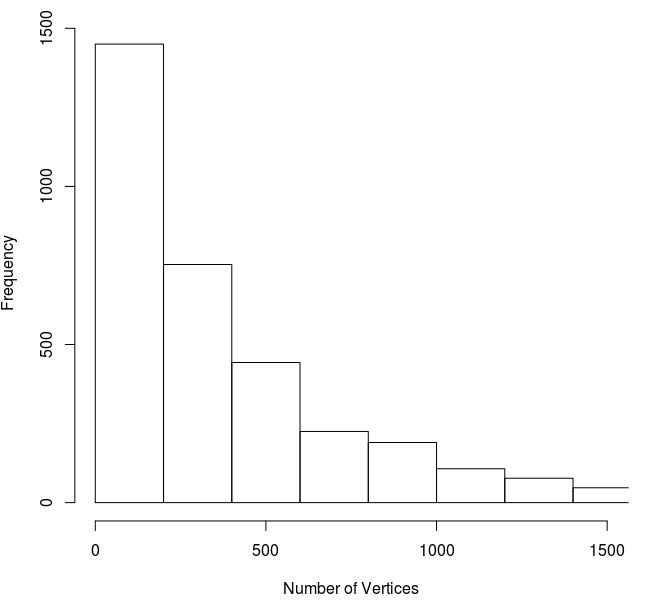
\includegraphics[width=3in]{num_vertices_histogram.png}
\label{fig:vertices-histogram}
\end{figure}

\begin{figure}[h!]
\caption{Average Runtime of Erickson and Edmonds-Karp Max-Flow Algorithms}
\centering
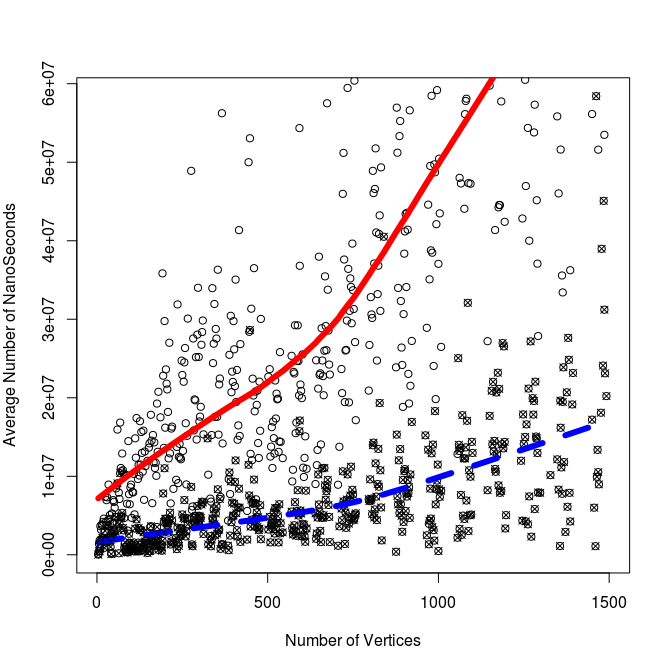
\includegraphics[width=5in]{maxflow_results_avg.png}
\label{fig:maxflow_avg}
\end{figure}

Figure \ref{fig:maxflow_avg} presents aggregated runtimes for graphs of different vertices. A total of 3414 trails were run, using graphs of size $n = 60$ to $n=3509$. However, the large majority of the graphs were of smaller sizes (i.e. $n < 1000$). Figure \ref{fig:vertices-histogram} presents a histogram of the number of vertices used by all the graphs in the trial. 

Interestingly, the Edmonds-Karp max-flow algorithm seems to perform significantly better on average than our implementation of Erickson's algorithm. This occurs for all of $n$ values for which we have data. Moreover, if one extrapolates the trend lines of Erickson's and Edmonds-Karp, one would not expect Erickson's to overtake Edmonds-Karp. The same relationship holds when one examines figure \ref{fig:maxflow_std} which presents the standard deviation of the runtimes for each algorithm. Unsurprisingly, the Erickson algorithm, which has a higher runtime, also has a higher runtime standard deviation. However, the higher runtime trend is surprising since Erickson's algorithm has better theoretical complexity than Edmonds-Karp.

\begin{figure}[h!]
\caption{Standard Deviation of Max-Flow Algorithm Runtimes}
\centering
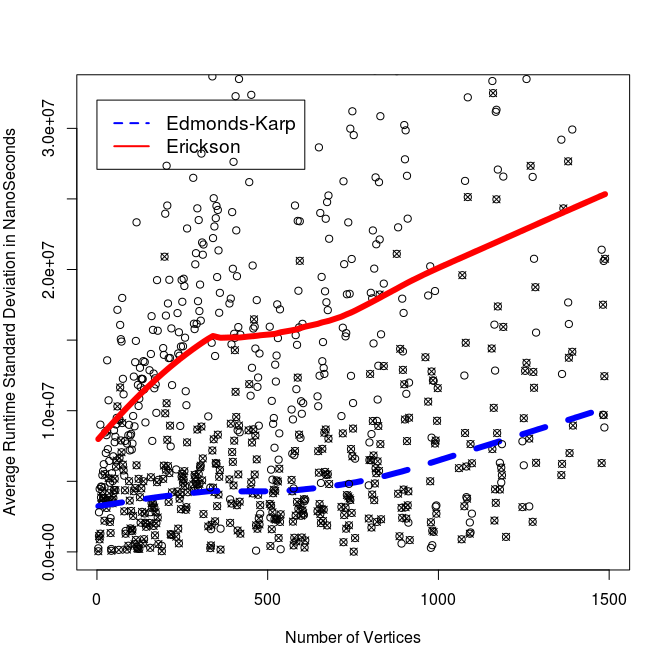
\includegraphics[width=5in]{maxflow_results_std.png}
\label{fig:maxflow_std}
\end{figure}

We can offer a number of hypotheses for this. First, it is possible that the graph sizes we used were too small to see the asymptotic advantage of Erickson's algorithm. This is likely, since we only generate graphs of size $n \leq 3509$ (due to memory constraints). 

Another possibility is that our implementation lacked efficiency. Since we emphasized modularity over speed, our implementation of Erickson's intialized a large number of objects in memory. Moreover, we decided to use a naive spanning tree data structure, which is $O(n)$ time per spanning tree operation instead of the $O(\log n)$ time obtained from the complicated but theoretically superior top-trees. In addition, our Dijkstra's algorithm did not implement a Fibonacci heap, so all decrease key operations were $O(\log n)$; however, our assumption that the queue would not significantly affect performance was correct, since the Djikstra portion of the algorithm empirically took less than 10\% of the total runtime for medium-sized graphs, and even less for the larger graphs.

What is the most likely cause of both the high standard deviation and poor performance of the implementation is the way that Java handles its memory.  Upon creation of the number of objects required for Erickson's algorithm to run on a graph of several thousand vertices, garbage collection in Java could devastate performance, and do so unpredictably.

\section{Conclusion}

This paper presented the Erickson algorthim from \cite{erickson2010} for finding max-flows in directed planar graphs. We presented motivation for the usefulness of this algorithm and summarized its main results, along with the algorithm's operation and runtime. Next, we implemented the Erickson, and compared this implementation to a standard Edmonds-Karp implementation in their ability to solve max-flows. 

We created SLOTIN, our own automated testing framework for examining max-flows in directed, planar graphs. The framework generates planar graphs, then generates comprehensive random flows, and tests the two algorithms on each max flow problem.  The results from the automated testing were found and analyzed, including using the number of lines of code as a benchmark for the amount of development time required. We found that the implementation of the Erickson algorithm performed substantially worse than the Edmonds-Karp implementation.  An efficient implementation would, in our opinion, have to 1) sacrifice too much developer time, 2) make too many strict sacrifices for efficiency over modularity, readability, and extensibility, and 3) and have to operate on problem sizes too large size to be useful in practice.

\section{Suggested Further Work}
Further pursuits of the analysis of the efficiency of Erickson's algorithm in practice should either explore territory not covered in this paper, or attempt to implement a ruthlessly efficient version of the algorithm in a language such as C.  Possible unexplored territory include the use of top trees in the main loop of the algorithm or more efficient queues in the Djikstra portion of the algorithm, although we do not expect the latter to yield much improvement.

\newpage

\begin{thebibliography}{9}

    \bibitem{erickson2010}
        Jeff Erickson.
       ``Maximum Flows and Parametric Shortest Paths in Planar Graphs.''
       \emph{Proceedings of the 21st Annual ACM-SIAM Symposium on Discrete Algorithms}.
       794-804.
       2010.

    \bibitem{dinitz1970}
        Yefim Dinitz.
        ``Algorithm for Solution of a Problem of Maximum Flow in a Network with Power Estimation.''
        \emph{Doklady Akademii nauk SSSR}.
        11: 1277-1280.
        1970.

    \bibitem{goldbergtarjan1986}
        Andrew Goldberg and Robert Tarjan.
        ``A New Approach to the Maximum Flow Problem.''
        \emph{Annual ACM Symposium on Theory of Computing}.
        Proceedings of the Eighteenth Annual ACM Symposium on Theory of Computing.
        136-146.
        1986.

    \bibitem{greigporteousseheult1989}
        D.M. Greig, B.T. Porteous, and A.H. Seheult.
        ``Exact Maximum A Posteriori Estimation for Binary Images.''
        \emph{Journal of the Royal Statistical Society. Series B (Methodological).}
        51(2): 271-279.
        1989.

    \bibitem{tarjanwerneck2005}
        R.E. Tarjan and R.F. Werneck.
        ``Self-Adjusting Top Trees.''
        \emph{Annual ACM Symposium on Discrete Algorithms.}
        Proceedings of the Sixteenth Annual ACM Symposium on Discrete Algorithms.
        812-822,
        2005.

    \bibitem{youngtarjanorlin1991}
        N.E. Young, R.E. Tarjan, and J.B. Orlin. 
        ``Faster Parametric Shortest Path and Minimum Balance Algorithms.''
        \emph{Networks.}
        21(2): 205-221.
        1991.

\end{thebibliography}

\end{document}
